% TriArchitect ICSE 2027 - TikZ Figures
% =============================================================
% Include this file in your main LaTeX document

\usepackage{tikz}
\usetikzlibrary{shapes.geometric, arrows.meta, positioning, calc, shadows, fit}

% =============================================================
% FIGURE 1: System Architecture
% =============================================================

\begin{figure}[t]
\centering
\begin{tikzpicture}[
    node distance=2.5cm,
    agent/.style={
        rectangle, rounded corners=8pt, 
        draw=black, line width=1pt,
        fill=blue!20, 
        minimum width=2.2cm, minimum height=1cm,
        font=\small\bfseries,
        drop shadow
    },
    tmg/.style={
        cylinder, shape border rotate=90,
        draw=black, line width=1.5pt,
        fill=orange!30,
        minimum width=2.5cm, minimum height=2cm,
        font=\small\bfseries,
        drop shadow
    },
    arrow/.style={
        ->, >=Stealth, line width=1pt
    },
    label/.style={
        font=\scriptsize, fill=white, inner sep=2pt
    }
]

% Center: Typed Migration Graph
\node[tmg] (tmg) {TMG};
\node[below=0.1cm of tmg, font=\tiny] {G = (V, E, τ, σ)};

% Agents orbiting TMG
\node[agent, above left=1.5cm and 2cm of tmg, fill=green!25] (arch) {Archeologist};
\node[agent, above right=1.5cm and 2cm of tmg, fill=blue!25] (arct) {Architect};
\node[agent, below=2cm of tmg, fill=red!25] (val) {Validator};

% Arrows with labels
\draw[arrow, color=green!60!black] (arch) -- node[label, pos=0.5, above, sloped] {Write} (tmg);
\draw[arrow, color=blue!60!black] (tmg) -- node[label, pos=0.4, above, sloped] {Read} (arct);
\draw[arrow, color=blue!60!black, dashed] (arct) -- node[label, pos=0.6, below, sloped] {Write} (tmg);
\draw[arrow, color=red!60!black] (tmg) -- node[label, pos=0.5, left] {Read} (val);

% Consensus Protocol box
\node[draw, dashed, rounded corners, 
      fit=(arch)(arct)(val)(tmg), 
      inner sep=15pt,
      label={[font=\small\itshape]below:Cyclic Consensus Protocol}] {};

% External inputs/outputs
\node[left=1cm of arch, font=\small] (input) {Java 8 Source};
\node[right=1cm of arct, font=\small] (output) {Java 17 Code};
\draw[arrow] (input) -- (arch);
\draw[arrow] (arct) -- (output);

% Docker container callout
\node[draw, fill=gray!10, rounded corners, 
      below right=0.5cm and 0.5cm of val,
      font=\tiny] {Docker Container\\JDK 17 + Maven};
\draw[arrow, dashed, gray] (val) -- ++(1.5, -0.8);

\end{tikzpicture}
\caption{TriArchitect System Architecture. The Typed Migration Graph (TMG) 
serves as persistent semantic memory. Archeologist populates the graph via 
static analysis. Architect reads migrated dependencies and writes proposals. 
Validator reads proposals and executes tests in isolated Docker containers.}
\label{fig:architecture}
\end{figure}

% =============================================================
% FIGURE 2: Cyclic Consensus Protocol Flow
% =============================================================

\begin{figure}[t]
\centering
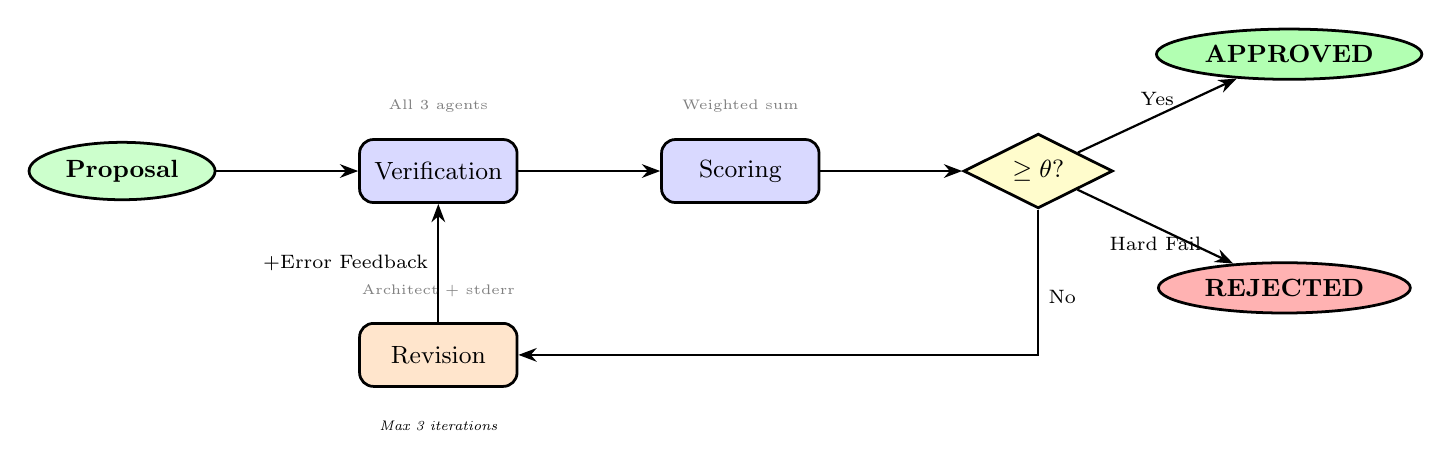
\begin{tikzpicture}[
    node distance=1.8cm,
    state/.style={
        rectangle, rounded corners=5pt,
        draw=black, line width=1pt,
        fill=blue!15,
        minimum width=2cm, minimum height=0.8cm,
        font=\small
    },
    decision/.style={
        diamond, aspect=2,
        draw=black, line width=1pt,
        fill=yellow!20,
        minimum width=1.5cm,
        font=\small
    },
    endpoint/.style={
        ellipse,
        draw=black, line width=1pt,
        fill=green!20,
        minimum width=1.5cm,
        font=\small\bfseries
    },
    arrow/.style={
        ->, >=Stealth, line width=0.8pt
    }
]

% Start
\node[endpoint] (start) {Proposal};

% Main flow
\node[state, right=of start] (verify) {Verification};
\node[state, right=of verify] (score) {Scoring};
\node[decision, right=of score] (check) {$\geq \theta$?};

% Outcomes
\node[endpoint, above right=1cm and 1.5cm of check, fill=green!30] (accept) {APPROVED};
\node[endpoint, below right=1cm and 1.5cm of check, fill=red!30] (reject) {REJECTED};

% Revision loop
\node[state, below=1.5cm of verify, fill=orange!20] (revise) {Revision};

% Arrows
\draw[arrow] (start) -- (verify);
\draw[arrow] (verify) -- (score);
\draw[arrow] (score) -- (check);
\draw[arrow] (check) -- node[above, font=\scriptsize] {Yes} (accept);
\draw[arrow] (check) -- node[below, font=\scriptsize] {Hard Fail} (reject);
\draw[arrow] (check) |- node[right, font=\scriptsize, pos=0.3] {No} (revise);
\draw[arrow] (revise) -- node[left, font=\scriptsize] {+Error Feedback} (verify);

% Iteration counter
\node[below=0.3cm of revise, font=\tiny\itshape] {Max 3 iterations};

% Agent labels
\node[above=0.2cm of verify, font=\tiny, color=gray] {All 3 agents};
\node[above=0.2cm of score, font=\tiny, color=gray] {Weighted sum};
\node[above=0.2cm of revise, font=\tiny, color=gray] {Architect + stderr};

\end{tikzpicture}
\caption{Cyclic Consensus Protocol flow. Proposals undergo verification by 
all three agents. Weighted scoring determines acceptance ($\theta = 0.85$). 
Rejection triggers error-informed revision by Architect (max 3 iterations).}
\label{fig:consensus}
\end{figure}

% =============================================================
% FIGURE 3: Results Bar Chart with Error Bars
% =============================================================

\usepackage{pgfplots}
\pgfplotsset{compat=1.18}

\begin{figure}[t]
\centering
\begin{tikzpicture}
\begin{axis}[
    ybar,
    bar width=12pt,
    width=0.95\columnwidth,
    height=6cm,
    ylabel={Test Passage Rate (\%)},
    symbolic x coords={GPT-5.1, GPT-5.1+RAG, Claude 4.5, MetaGPT, MigMiner, TriArch},
    xtick=data,
    xticklabel style={rotate=30, anchor=east, font=\small},
    ymin=0, ymax=100,
    ytick={0,20,40,60,80,100},
    ymajorgrids=true,
    grid style={dashed, gray!30},
    legend style={at={(0.02,0.98)}, anchor=north west, font=\small},
    error bars/.cd,
        y dir=both,
        y explicit,
]

% Test Passage Rate with 95% CI error bars
\addplot[
    fill=blue!60,
    error bars/.cd,
        y dir=both,
        y explicit,
] coordinates {
    (GPT-5.1, 58.4) +- (0, 2.5)
    (GPT-5.1+RAG, 65.2) +- (0, 2.3)
    (Claude 4.5, 67.1) +- (0, 2.2)
    (MetaGPT, 70.3) +- (0, 2.0)
    (MigMiner, 76.2) +- (0, 1.9)
    (TriArch, 87.3) +- (0, 1.5)
};

\end{axis}
\end{tikzpicture}
\caption{Test Passage Rate comparison across baselines. Error bars show 
95\% confidence intervals ($n=1000$, 5 runs). TriArchitect achieves 87.3\% 
vs. 58.4\% for GPT-5.1 single-agent—a 28.9 percentage point improvement.}
\label{fig:results}
\end{figure}

% =============================================================
% FIGURE 4: Grouped Bar Chart (Alternative)
% =============================================================

\begin{figure}[t]
\centering
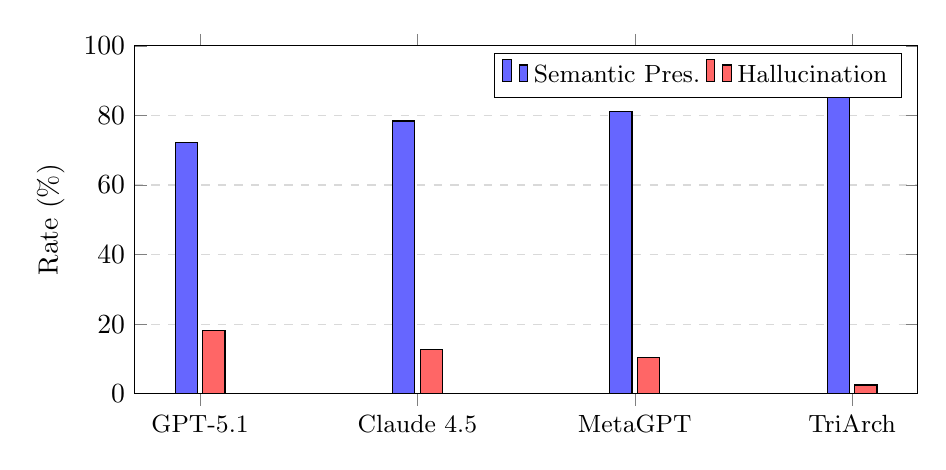
\begin{tikzpicture}
\begin{axis}[
    ybar,
    bar width=8pt,
    width=0.95\columnwidth,
    height=6cm,
    ylabel={Rate (\%)},
    symbolic x coords={GPT-5.1, Claude 4.5, MetaGPT, TriArch},
    xtick=data,
    xticklabel style={font=\small},
    ymin=0, ymax=100,
    ymajorgrids=true,
    grid style={dashed, gray!30},
    legend style={at={(0.98,0.98)}, anchor=north east, font=\small},
    legend columns=2,
]

% Semantic Preservation
\addplot[fill=blue!60] coordinates {
    (GPT-5.1, 72.3)
    (Claude 4.5, 78.4)
    (MetaGPT, 81.2)
    (TriArch, 94.2)
};

% Hallucination Rate (inverted for clarity: lower is better)
\addplot[fill=red!60] coordinates {
    (GPT-5.1, 18.2)
    (Claude 4.5, 12.8)
    (MetaGPT, 10.4)
    (TriArch, 2.5)
};

\legend{Semantic Pres., Hallucination}

\end{axis}
\end{tikzpicture}
\caption{Semantic Preservation vs. Hallucination Rate. TriArchitect achieves 
94.2\% semantic preservation while reducing hallucination to 2.5\%.}
\label{fig:grouped}
\end{figure}
